%-------------------------------------------------------------------------
\section{Evaluation} 
\label{sec:tracker-eval}

\subsection{Tracker configuration}

To better evaluate how each component contributes to the tracker in videos under various conditions, we use three different configurations of our tracking system, based on the inputs used. BG uses background subtraction and optical flow, DET uses the object detector and optical flow, and BG+DET uses all three inputs. 
We also run several state-of-the-art trackers, including KCF \cite{henriques2015high}, STRUCK \cite{hare2011struck}, ASMS \cite{vojir2014robust}, DAT\cite{possegger2015defense}, staple \cite{bertinetto2016staple}, MEEM \cite{zhang2014meem} and SRDCF \cite{danelljan2015learning} as baselines. 
%STRUCK is the top-scorer on a variety of videos a recent (2015) benchmark paper \cite{wu2015object}. 
Since all these trackers require manual initialization (namely human input), they are not able to be compared with our tracker directly. Instead, we can only partially evaluate them by providing manual initialization, see \S\ref{subsec:tracker-eval-overall}. By carefully selected manual initialization, the comparison here is in favor of the baselines.

%-------------------------------------------------------------------------
\subsection{Evaluation metrics}

Given a set of generated and ground truth object trajectories, usually represented by a sequence of rectangular bounding boxes, we desire one or more performance metrics that capture the accuracy of the proposed system. Aspects that need to be captured include 1) tracking duration---if a ground truth trajectory of an object contains N frames, for how many of these frames does the system track the object, 2) recall---how many of the ground truth trajectories were represented in the tracking result, 3) precision---what proportion of tracking results had a corresponding trajectory, as well as 4) the overlap between the tracking result and the ground-truth.

Note that our problem does not fit into common multi-object tracking setting, since moving objects are tracked individually, instead of being modeled globally. Common metrics such as MOTA \cite{bernardin2008evaluating} would generate a meaningless number since we could have potentially more objects tracked than ground truth.

As the first step, we match each ground truth to a tracking result, by maximizing the accumulated overlap ratio $r$, 
\begin{align}
    r=\frac{\sum_t{(S_t^{gt}\cap S_t^{traj})}}{\sum_t{(S_t^{gt}\cup S_t^{traj})}},
    \label{eq:ratio-all}
\end{align}
where $S_t^{gt}$ and $S_t^{traj}$ are ground truth and trajectory box areas at frame $t$, respectively. Note that the sum is computed over the union of trajectory and ground truth lifetime. 
%For example, the ground truth appears from frame 1 to 100, while object tracker lasts from frame 20 to 150, the denominator is summed over frame $1\sim150$. 
%Suppose we have two trajectories overlap with the same ground truth, one tracks well in a short period while the other tracks almost as well, but for a longer duration. 
\ref{eq:ratio-all} ensures the ground truth is matched to a longer trajectory with reasonable coverage. 
Additionally, to filter some spurious objects slightly touched the ground truth, we also require any match to have more than $30\%$ overlap on at least one frame, where the value is set experimentally.

%On the other hand, it is more than a collection of manually initialized single-object trackers. The falsely tracked objects due to automatic initialization should be minimized and one-to-one matching of automatically generated trajectories and ground truth should be made before any accuracy evaluation is performed.
%Several metrics have been proposed in the past, including Fscore \cite{kwon2009tracking}, deviation \cite{sanin2012shadow}, and object tracking accuracy (MOTA) \cite{bernardin2008evaluating}. 

%While these work for pure tracking evaluation, where initialization and termination (usually the end of the video clip) is given, these are not well suited to our dataset. 
\subsection{Object-level evaluation} 
\label{subsec:tracker-eval-count}

Given the matched results, we can calculate the proportion of ground truth trajectories that were matched to the tracking result (recall), and the proportion of tracking results that had a matching trajectory (precision), for our three trackers and two types of videos. 
\ref{fig:kf-eval-count-low} and \ref{fig:kf-eval-count-high} show the results in absolute numbers, also to provide some perspectives on the scale of the evaluation. The true positives are those correctly tracked objects and false positives are noisy objects. Our best tracker configuration, BG+DET, achieves $81\%$ recall and $87\%$ precision on our low resolution, simple videos, and $65\%$ recall, $57\%$ precision on the high-resolution, complex scenes. Here, the majority of failures in the complex scenes were due to complicated interactions and heavy occlusion throughout the scene, where vehicles were only partially visible. Currently, we do not split such merged objects into their constituent parts; we leave this for future work. 

Comparing the three configurations, we see that the detector performs quite poorly on the low-resolution scenes, due to small and poor quality imagery where it is sometimes difficult even for a person to correctly identify an object as a vehicle. By contrast, background subtraction does quite well on these uncomplicated scenes. For the more higher resolution complex scenes, the detector performs well, while the background subtraction model struggles and largely introduces noise.

% \setlength{\belowcaptionskip}{-10pt}
\begin{figure}
  \centering
    % \begin{minipage}{0.45\linewidth}
    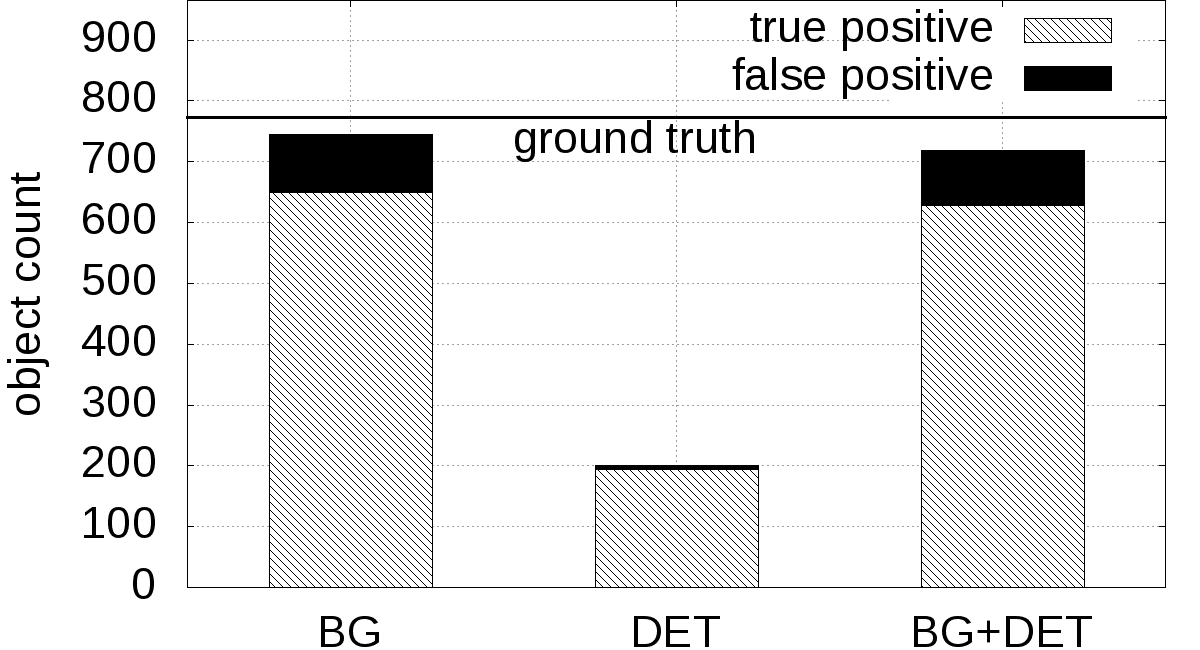
\includegraphics[width=\linewidth]{./img/evaluation/count_lowRes.png}
    \caption{Tracked object count on low resolution, less complex scenes.}
    \label{fig:kf-eval-count-low}
    %\vspace{-0.5em}
    % \end{minipage}
\end{figure}
\begin{figure}
    \centering
    % \begin{minipage}{0.45\linewidth}
    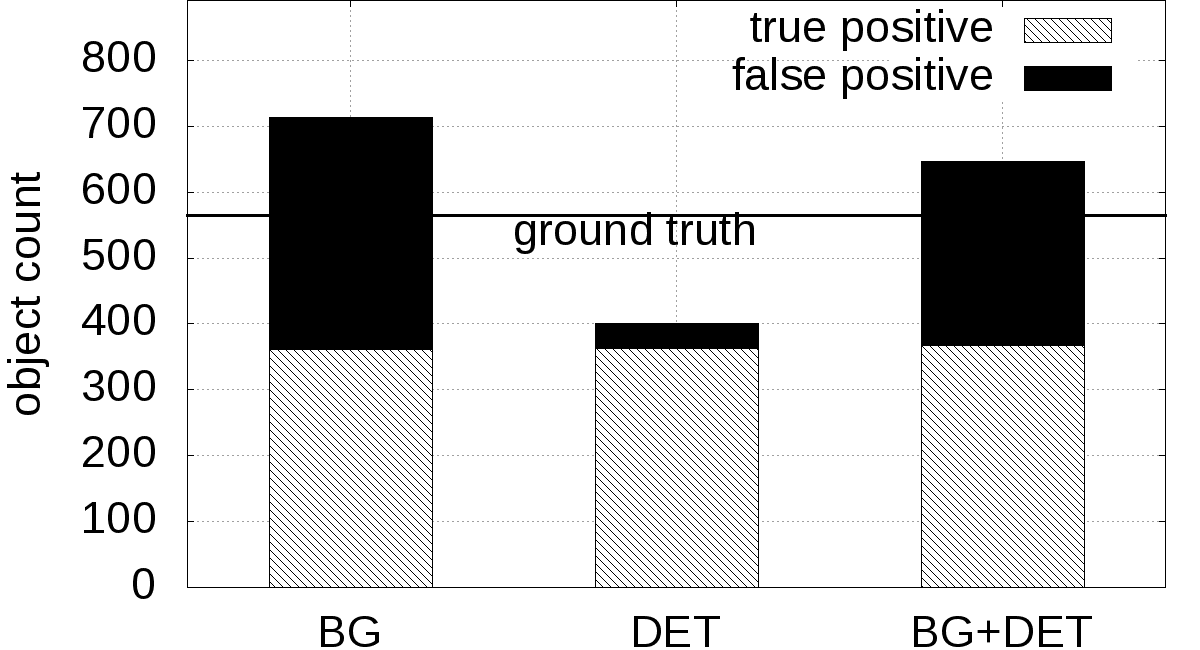
\includegraphics[width=\linewidth]{./img/evaluation/count_highRes.png}
    \caption{Tracked object count on high resolution, more complex scenes.}
    % \end{minipage}
    % \caption{Tracked object count under different tracker settings.}
    \label{fig:kf-eval-count-high}
\end{figure}
%-------------------------------------------------------------------------
% \subsubsection{Overlap area during match}
% \begin{figure*}
% \begin{minipage}{0.33\textwidth}
%   \includegraphics[width=\linewidth]{./img/initOverlap/overlapArea_lowRes.pdf}
%       \subcaption{Simple low resolution videos.}
%   \label{fig:area_lowRes}
% \end{minipage}
% \begin{minipage}{0.33\textwidth}
%   \includegraphics[width=\linewidth]{./img/initOverlap/overlapArea_highRes.pdf}
%       \subcaption{Complex high resolution videos.}
%   \label{fig:area_highRes}
% \end{minipage}
% \begin{minipage}{0.33\textwidth}
%   \includegraphics[width=\linewidth]{./img/initOverlap/overlapArea_night.pdf}
%       \subcaption{Night videos.}
%   \label{fig:area_night}
% \end{minipage}
%   \caption{Mean overlapped area of every object on each frame.}
% \end{figure*}
%-------------------------------------------------------------------------
% \subsubsection{Deviation during match}
% \begin{figure*}
% \begin{minipage}{0.33\textwidth}
%     \includegraphics[width=\linewidth]{./img/initDeviation/deviation_lowRes.pdf}
%     \subcaption{Simple low resolution videos.}
%     \label{fig:deviation_lowRes}
% \end{minipage}
% \begin{minipage}{0.33\textwidth}
%     \includegraphics[width=\linewidth]{./img/initDeviation/deviation_highRes.pdf}
%     \subcaption{Complex high resolution videos.}
%     \label{fig:deviation_highRes}
% \end{minipage}
% \begin{minipage}{0.33\textwidth}
%     \includegraphics[width=\linewidth]{./img/initDeviation/deviation_night.pdf}
%     \subcaption{Night videos.}
%     \label{fig:deviation_night}
% \end{minipage}
%     \caption{Mean center deviation of every object on each frame.}
% \end{figure*}
%-------------------------------------------------------------------------


\subsection{Pixel-level evaluation during entire lifetime} 
\label{subsec:tracker-eval-overall}

We are also interested in evaluating how well the tracker follows objects in the scene. For example, as one of our motivating application, accurate tracking is necessary for correct turning movement classification, as \ref{fig:screenshots}\subref{subfig:193402} illustrates.
While there exists no similar work or benchmark that incorporates automatic initialization, we can only partially compare our system to prior work. Here, we modify our tracker to accept manual initialization. Both our modified trackers and the baseline trackers are initialized with boxes extracted from ground truth. These ``initialized'' trackers are then evaluated along with our automatically initialized trackers. Note that the experiment is designed in favor of those manually initialized trackers, since the initialization boxes are from ground truth and perfectly match the object in the scene.

To accept manual initialization in scenes with significant scale change, each tracker is initialized with the first box of ground truth larger than a threshold: 
\begin{align}
    S_{thresh}=\left[\text{max}(S^{gt})-\text{min}(S^{gt})\right]*s + \text{min}(S^{gt}),
    \label{eq:thresh}
\end{align}
where $\text{max}(S^{gt})$ and $\text{min}(S^{gt})$ are the maximal and minimal ground truth areas along the sequence. $s\in \{0, 0.2, \dots, 1.0\}$, corresponds to the minimum fraction of the maximum object size at which initialization may occur. Note $s$ only affects objects that enter with an increasing size; while shrinking objects would be initialized upon appearance regardless of the threshold. 
Tracking is terminated at the last frame of ground truth. 
% Different with \cite{Wu_2013_CVPR}, we do not do any re-initialization after failure, since we are evaluating one-time tracking.
We arrived at this design as some trackers tend to perform poorly when initialized by small images, yet delaying initialization until the object grows large can result in arbitrarily shortened trajectory.

\ref{fig:kf-eval-overlap-low} and \ref{fig:kf-eval-overlap-high} compare the overlap ratio of our three tracker configurations both with manual and automatic initialization (horizontal lines), as well as the overlap ratio of several other trackers on our high- and low-resolution datasets. 
The x-axis is the initialization threshold $s$ in \ref{eq:thresh}, and the y-axis is the overlap ratio $r$ from \ref{eq:ratio-all}, averaged over all objects.
This is computed from the first to the last frame of ground truth for the manually initialized and terminated trackers. While for our automatic trackers, it is computed over the union of tracking and ground truth lifetimes. This accounts for both tracking accuracy and lifetime, as we illustrated before.

% \setlength{\belowcaptionskip}{-10pt}
\begin{figure}
  \centering
  % \begin{minipage}{0.45\linewidth}
    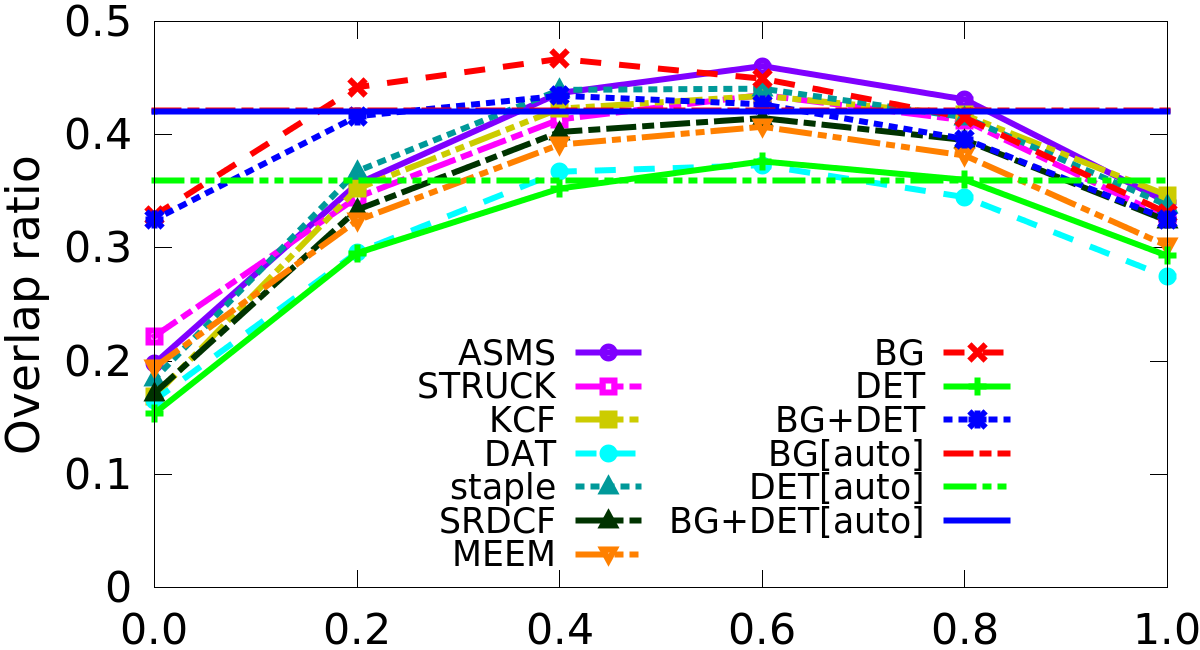
\includegraphics[width=\linewidth]{./img/evaluation/overlapRatioAllPerObj_lowRes.png}
    \caption{Overall overlap ratio on low resolution, less complex scenes.}
    \label{fig:kf-eval-overlap-low}
    %\vspace{-0.5em}
    % \end{minipage}
    % \begin{minipage}{0.45\linewidth}
\end{figure}
\begin{figure}
    \centering
    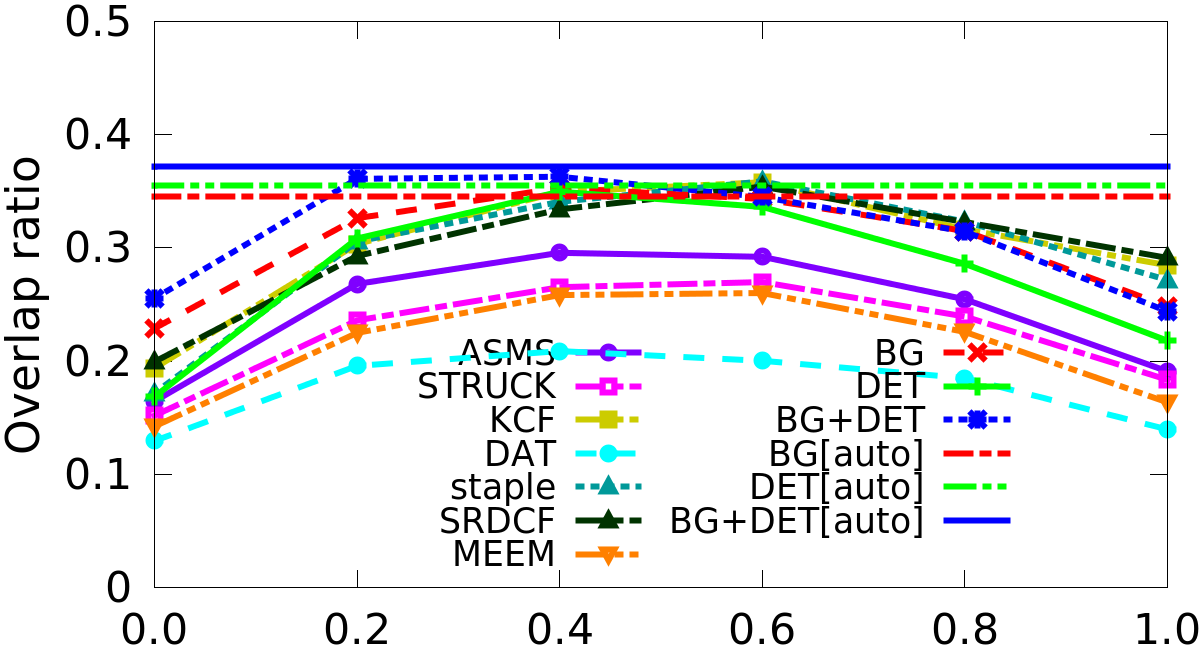
\includegraphics[width=\linewidth]{./img/evaluation/overlapRatioAllPerObj_highRes.png}
    \caption{Overall overlap ratio on high resolution, more complex scenes.}
    % \end{minipage}
    % \caption{Overall overlap ratio.}
    \label{fig:kf-eval-overlap-high}
\end{figure}

The shape of the curves for the initialized trackers captures the trade-off between early-and-inaccurate, vs. late-but-accurate initialization. Overall, our BG-based trackers handily outperform other trackers when manual initialization and termination is provided. More importantly, the auto-initialized BG trackers essentially meet the performance of other trackers on the simple videos, and significantly outperform them on the complex videos. We hypothesize that the automatic initialization allows the tracker to better adapt to individual vehicles vs. the constant threshold set for manual initialization. Additionally, consistent with our conclusion in \S\ref{subsec:tracker-eval-count}, detector dominates the tracking update on high resolution videos, while background subtraction plays its role on low resolution videos.

\subsection{Pixel-level evaluation during tracked period} 
\label{subsec:tracker-eval-acc}

Then we focus on the performance during only the tracked period. Borrowed from standard single object tracking measurement, we show the success plot for trackers for two video groups, in \ref{fig:kf-eval-success-low} and \ref{fig:kf-eval-success-high}. Different from above, we compute the success frame rate from the initialization frame, instead of entire ground truth sequence. The performance is measured by the area under the curve. By \ref{fig:kf-eval-overlap-low} and \ref{fig:kf-eval-overlap-high} we see overlap ratio between 0.2 and 0.6 is a good balance of tracking accuracy and trajectory completeness, we hereby show results of initialization threshold of 0.4 here.
Our automatic trackers significantly outperform other trackers with manual initialization. This demonstrates that proper initialization is critical to the tracking performance and similar conclusion about the contribution of each tracking component can be drawn.

% \setlength{\belowcaptionskip}{-10pt}
\begin{figure}
  \centering
  % \begin{minipage}{0.45\linewidth}
    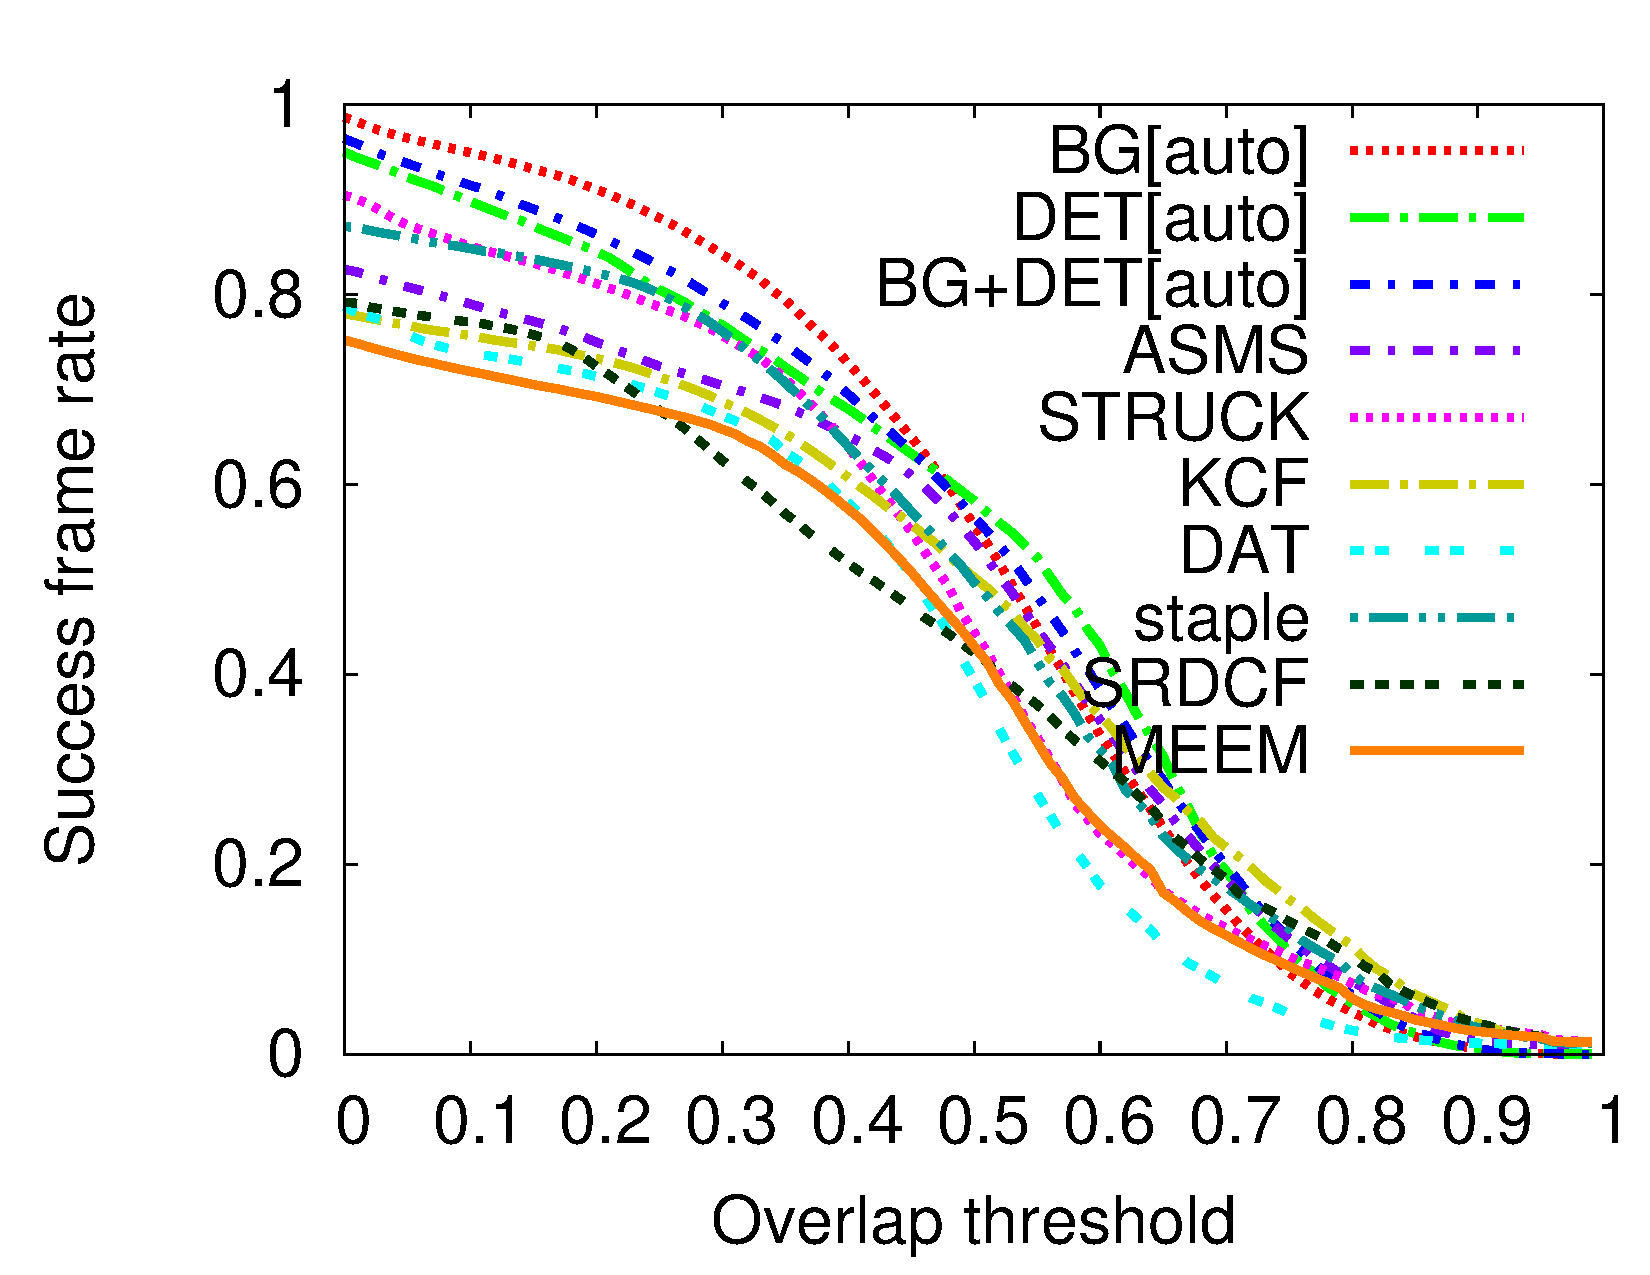
\includegraphics[width=\linewidth]{./img/evaluation/success_lowRes.pdf}
    \caption{Success plot of low resolution, less complex scenes.}
    \label{fig:kf-eval-success-low}
\end{figure}
    %\vspace{-0.5em}
% \end{minipage}
% \begin{minipage}{0.45\linewidth}
\begin{figure}
  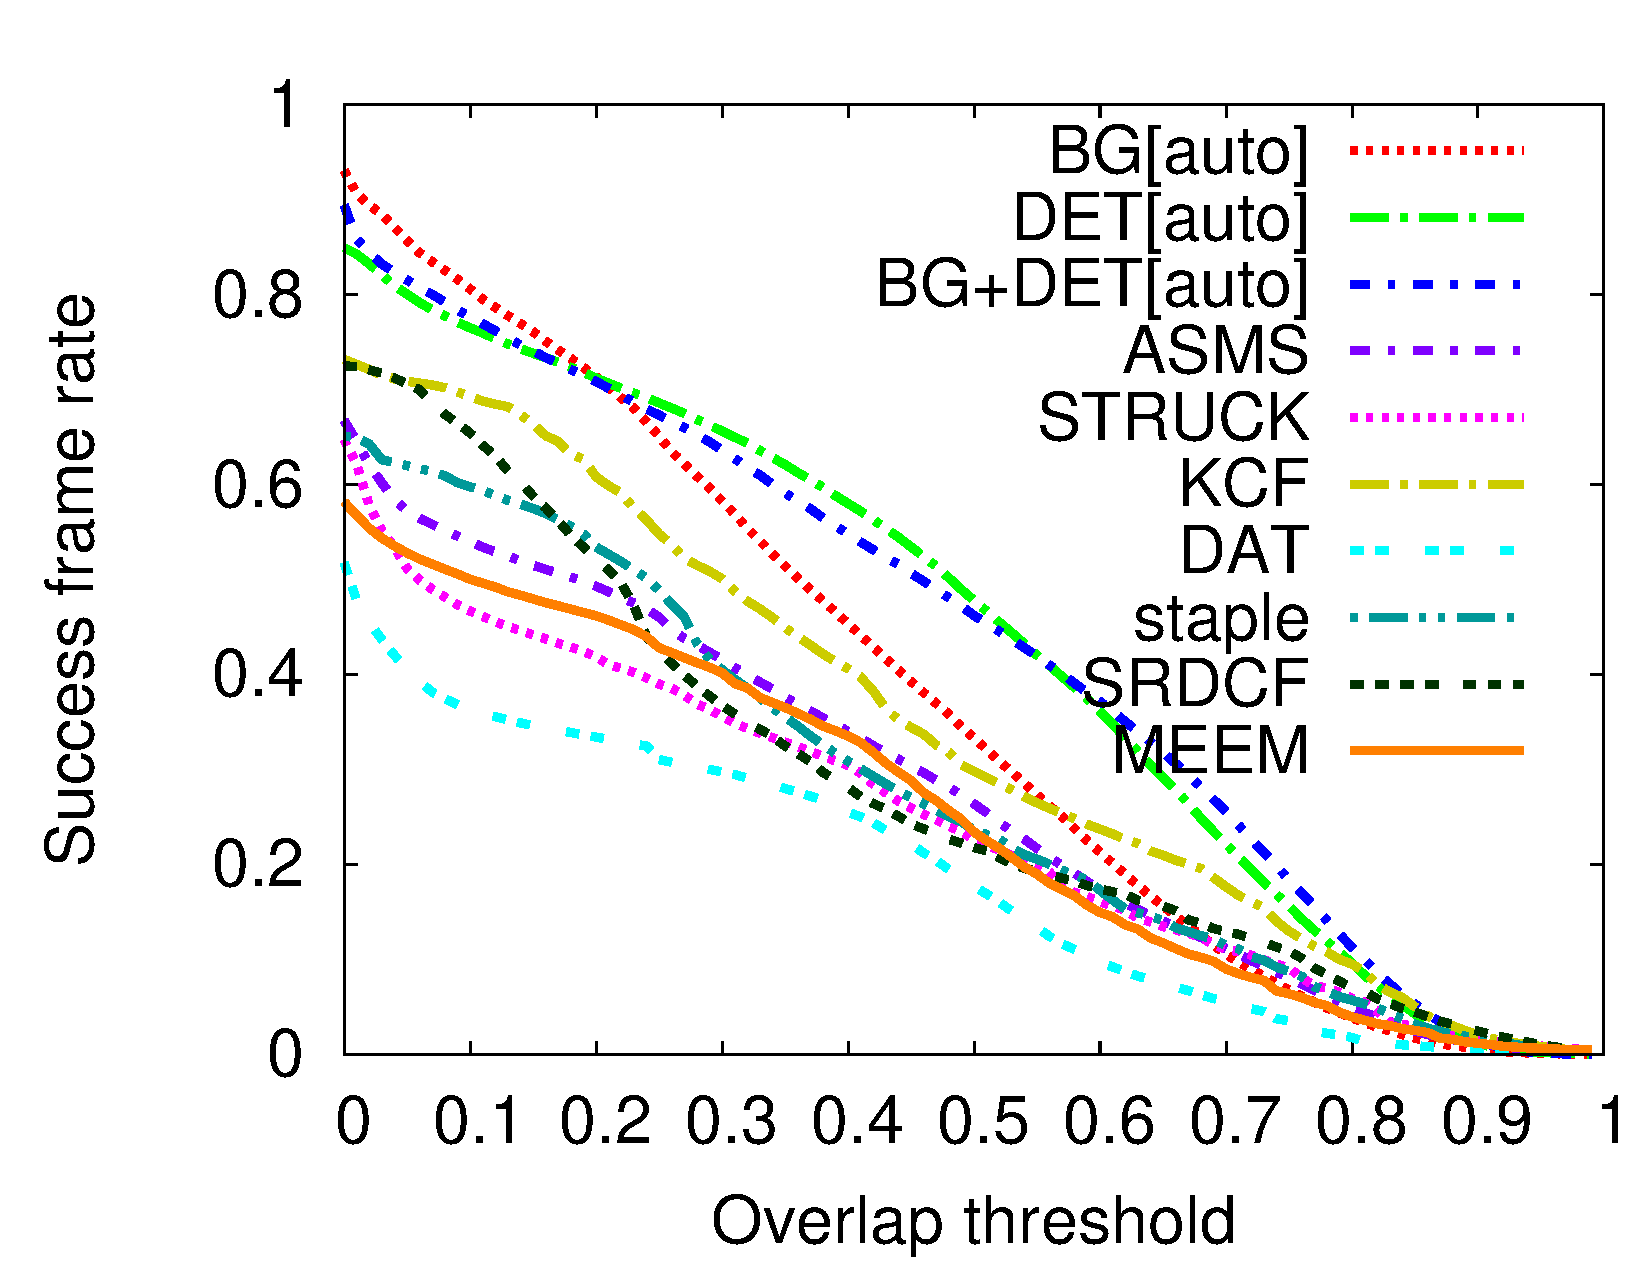
\includegraphics[width=\linewidth]{./img/evaluation/success_highRes.pdf}
    \caption{Success plots of high resolution, more complex scenes.}
% \end{minipage}
  % \caption{Success plots.}
  \label{fig:kf-eval-success-high}
\end{figure}

%% \subsection{Overlap ratio during tracking}\label{subsection:matchRatio}
%% As a supplement, we present the tracking accuracy during the tracking process, thus ignoring the trade-off between duration and accuracy. The only difference compared with the previous subsection is that the overlap ratio $r$ is computed during tracking only: from the initialization frame to last frame of ground truth, instead of from the first frame of ground truth.

%% In Figs \ref{fig:ratio_lowRes}--\ref{fig:ratio_highRes}, the overlap ratio grows with the initialization threshold, then largely levels out rather than drop as in Figs \ref{fig:ratioAll_lowRes}--\ref{fig:ratioAll_highRes}. Thus tracking performance improves with better initialization up to some point. With thresholds of 1.0, a small drop is recorded in some curves---this is likely noise due to the very short tracking duration under that setting. 

%% Consistent with previous results, BG and BG+DET are very similar and the most accurate. Fig \ref{fig:ratioMatch}(\subref{subfig:ratio_lowRes}) shows more similar trend with Fig \ref{fig:ratioAll}, indicating that initialization with small size may affect the tracking accuracy.

%% Based on Fig \ref{fig:ratioMatch} and Fig \ref{fig:ratioAll}, we conclude that $s$ between 0.2--0.6 is a good balance between accuracy and lifetime and our automatic tracker achieves almost the same performance in terms of such balance.
%% \begin{figure}
%%   \centering
%%  \includegraphics[height=1.8in]{./img/initOverlapRatioMatch/overlapRatioMatch_lowRes.pdf}
%%      \caption{Overlap ratio during the tracking process only, on low resolution videos.}
%%  \label{fig:ratio_lowRes}
%% \end{figure}
%% \begin{figure}
%%         \includegraphics[height=1.8in]{./img/initOverlapRatioMatch/overlapRatioMatch_highRes.pdf}
%%      \caption{Overlap ratio during the tracking process only, on high resolution videos.}
%%  \label{fig:ratio_highRes}
%% \end{figure}
\begin{figure}
    \centering
    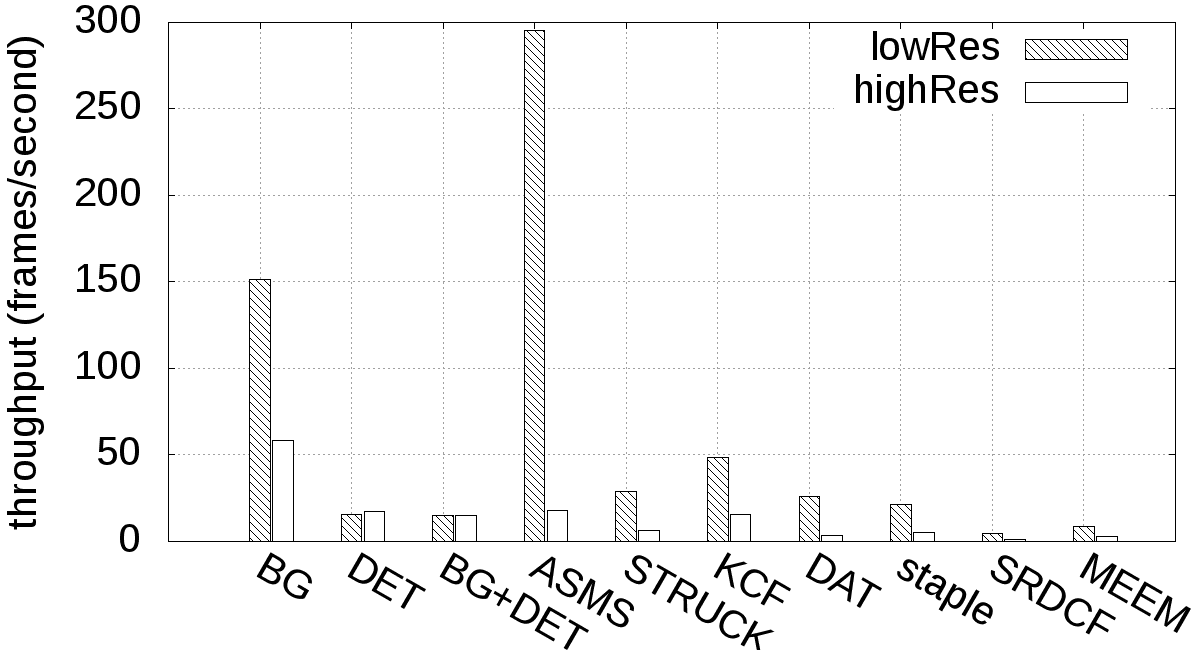
\includegraphics[width=\linewidth]{./img/evaluation/throughputInit_group.png}
   \caption{Tracker throughput on different resolution videos.}
    \label{fig:kf-eval-throughput}
\end{figure}

\subsection{Throughput}
Finally, we explore the throughput of trackers on different resolution videos, as shown in \ref{fig:kf-eval-throughput}.
The evaluation was done on a Linux desktop with an Intel Core i7-3770 3.40GHz processor and a GeForce GTX TITAN X GPU.
According to these results, BG significantly outperforms 6 out of 7 baseline trackers, with around 5$\times$ throughput improvement compared with real time (about 30 fps). Interestingly, ASMS outperforms our BG tracker on low resolution videos, however, it becomes 17$\times$ slower once it is applied on high resolution videos. Although the use of the object detector (DET, BG+DET) makes the tracker slower, they are the only ones that maintain a similar frame rate on both low- and high resolution videos near real time, showing good scalability of resolution.
% it is able to maintain frame rate, with the intermittent detector versions going dramatically faster. 
%The difference between low and high resolution videos becomes negligible when the detection interval decreases. We believe the reason behind this is that the GPU is not fully utilized by the detector on low resolution videos. %Overall BG is more suitable for time-critical application, while DET and BG+DET have high tolerance of resolutions.

